\clearpage
\section{Recognizing Ministers and Vestments}
\subsection*{Distinct Ministers in the Postconciliar Sanctuary}
The General Instruction of the Roman Missal distinguishes ordained ministers, instituted lay ministries, extraordinary ministers of Holy Communion, and altar servers. Each office carries its own vesture and handling boundary, and none is interchangeable with another.

{\footnotesize\begin{longtable}{>{\raggedright\arraybackslash}p{0.20\linewidth}>{\raggedright\arraybackslash}p{0.28\linewidth}>{\raggedright\arraybackslash}p{0.45\linewidth}}
\toprule
\textbf{Minister} & \textbf{Appointed vesture} & \textbf{Sanctuary and handling role} \\
\midrule
\endhead
\textbf{Bishop (Episcopus)} & Alb, cincture, amice (if needed), pectoral cross, straight stole, pontifical dalmatic (at major pontifical Masses), chasuble or cope, miter, ring, crosier. & Principal liturgist of the diocese (GIRM 92); dedicates fixed altars, consecrates Sacred Chrism, blesses Holy Oils, judges tabernacle placement (GIRM 315), ordinary minister of Holy Communion. \\
\textbf{Priest (Presbyter)} & Alb, cincture (unless fitted), amice (if collar exposed), straight vertical stole, chasuble at Mass (GIRM 337); cope outside Mass (GIRM 341); choir dress or cassock and surplice when not concelebrating (RS 128). & Confects the Eucharist in the person of Christ the Head (GIRM 93; RS 154); blesses vessels and vestments (GIRM 333, 335); ordinary minister of Holy Communion; consumes remaining Precious Blood and purifies sacred vessels. \\
\textbf{Deacon (Diaconus)} & Alb, cincture (unless fitted), amice (if collar exposed), diagonal stole over left shoulder fastened at right hip (GIRM 340), dalmatic worn over stole (GIRM 338; omission discouraged by RS 125). & Carries Book of the Gospels and proclaims Gospel; prepares altar and chalice; elevates chalice at doxology; ordinary minister of Holy Communion and especially of the chalice (GIRM 182); purifies vessels (GIRM 279). \\
\textbf{Instituted Acolyte (Acolythus institutus)} & Alb (common garment of instituted ministers, GIRM 336) or other dignified attire in U.S. (GIRM 339); never stole, dalmatic, or chasuble (RS 126). & Layperson formally instituted by the bishop (Ministeria quaedam 1972; CIC can. 230 as amended by Spiritus Domini 2021). Assists at altar; extraordinary minister of Holy Communion ex officio; uniquely among laity may purify sacred vessels (GIRM 279; USCCB Norms 53). \\
\textbf{Instituted Lector (Lector institutus)} & Alb (GIRM 336) or dignified attire in U.S. (GIRM 339); never stole, dalmatic, or chasuble (RS 126). & Layperson formally instituted by the bishop (CIC can. 230). Carries Book of the Gospels in entrance procession only in the deacon's absence (GIRM 120d, 194); proclaims Scripture readings other than the Gospel and intentions of Universal Prayer. \\
\textbf{Extraordinary Minister of Holy Communion (EMHC)} & Dignified lay attire or alb per diocesan directive (GIRM 339); never clerical vestments or stole (RS 126). & Deputed layperson acting strictly in genuine pastoral necessity (GIRM 100, 162; RS 155--158). Approaches altar only after the priest communicates (USCCB Norms 38); distributes Communion from handed vessels; may not purify sacred vessels (GIRM 279; Oct 2006 CDWDS decision; USCCB Norms 53). \\
\textbf{Altar Server (Ministrans)} & Alb (with cincture if unfitted) or black cassock with white surplice (never surplice without cassock, CE 65) or other dignified attire approved in U.S. (GIRM 339); never clerical insignia. & Non-instituted lay server (GIRM 107; RS 47). Carries processional cross, candles, thurible, boat, bells, cruets, lavabo, and aspersorium; holds Missal or Book of the Chair; brings unconsecrated vessels at Preparation of Gifts. Never opens tabernacle, carries consecrated species, carries Book of Gospels in procession, or purifies vessels. \\
\textbf{Sacristan (Sacrista)} & Ordinary dignified attire in the sacristy (vested in alb or cassock and surplice only when also exercising a sanctuary ministry). & Prepares sacred vessels, linens, liturgical books, vestments, candles, and credence table before Mass and sees to orderly care, sacrarium first-rinsing of linens (RS 120), and storage after Mass (GIRM 105). \\
\bottomrule
\end{longtable}}

\clearpage
\PCDPlateHeader{Plate VIII --- Ordained Vesture at Mass}{Standing figures to common scale; insets not to scale}
\ifdefined\TriptychPrintEdition
\begin{center}
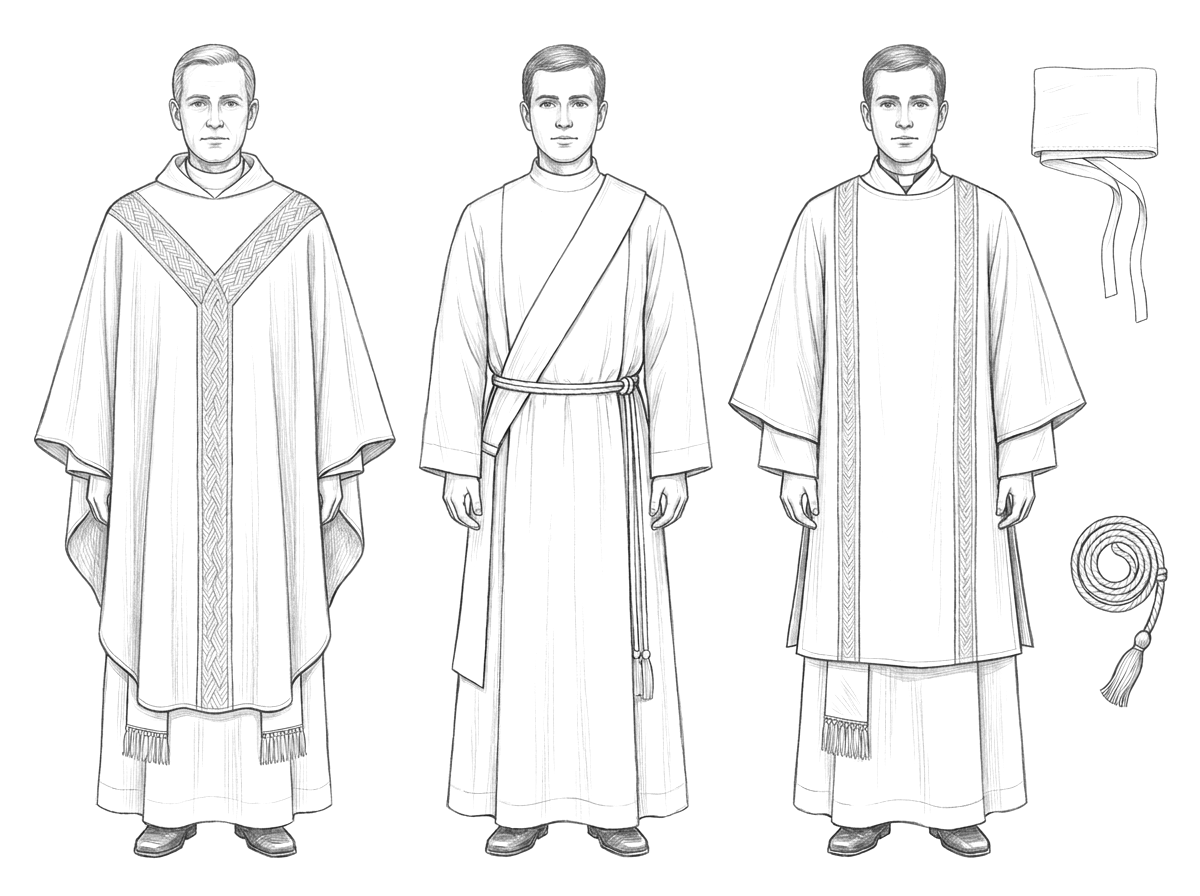
\includegraphics[width=0.92\linewidth,height=3.55in,keepaspectratio]{liturgy/roman-rite/postconciliar/2008-latin-2011-us-english/reference/roman-sanctuary-dictionary/shared/artwork/graphite/pc-art-08-priest-deacon-vesture.png}
\end{center}
\PCDPositionKey{Left: Priest in Alb, Amice, straight vertical Stole, and Y-orphrey Chasuble; center: Deacon in Alb, Cincture, and diagonal Stole from left shoulder to right hip without dalmatic; right: Deacon in Alb and sleeved Dalmatic worn over the diagonal Stole (fringed tip peeking at deacon's right side); far right insets: folded Amice with ties (top) and coiled tasseled Cincture (bottom).}
\else
\textbf{Visual Plate Summary (Plate VIII --- Ordained Vesture at Mass, Standing figures to common scale; insets not to scale):} Worn monochrome graphite vestment study comparing priest and deacon at common scale: left, a priest vested in ankle-length white alb, amice at collar, straight vertical stole ends visible below a flowing Gothic chasuble with Y-shaped orphrey; center, a deacon in white alb and tied cord cincture wearing his stole diagonally from left shoulder across the chest to his right hip; right, a deacon vested in a wide-sleeved dalmatic with vertical clavi stripes worn over the diagonal stole, whose fringed end peeks below the deacon's right hem; far right margin insets show a folded rectangular amice with cloth ties above and a coiled tasseled cincture below.

\textbf{Reading order and object placement:} Left: Priest in Alb, Amice, straight vertical Stole, and Y-orphrey Chasuble; center: Deacon in Alb, Cincture, and diagonal Stole from left shoulder to right hip without dalmatic; right: Deacon in Alb and sleeved Dalmatic worn over the diagonal Stole (fringed tip peeking at deacon's right side); far right insets: folded Amice with ties (top) and coiled tasseled Cincture (bottom).
\fi

\label{pc-obj-alb}
\PCDEntryHead{Alb}{Alba}{required}{N31}
\PCDField{Also called}{White Tunic; \textit{Tunica alba}}
If your parish vests altar servers in albs (US GIRM 339), pick one that reaches your ankles without brushing the floor so you never trip on sanctuary steps. Make sure ordinary shirt collars and long sleeves stay neatly covered, fasten a cincture at the waist if the alb is not tailored to fit smoothly (GIRM 336), and hang your alb straight on a hanger after Mass. Remember that servers, instituted acolytes, instituted lectors, and extraordinary ministers of Holy Communion never wear a stole over an alb (RS 126).

\PCDField{Where to look on the plate}{Worn beneath chasuble, diagonal stole, and dalmatic across all three figures (Plate VIII), and under cope and humeral veil (Plate IX)}
\PCDField{Handling boundary}{\textbf{Server handles directly.} Altar servers may wear a clean white alb hemmed at ankle height (tied with a cincture if unfitted) where parish custom appoints it under US GIRM 339, hanging it neatly after Mass and never wearing clerical insignia over it (RS 126). (Ordinary ministers: Bishop, Priest, Deacon, Instituted acolyte, Instituted lector, Extraordinary minister of Holy Communion, Altar server.)}
\PCDSafety{Choose an alb whose hem clears your shoes cleanly at ankle height; an overly long hem catches on sanctuary steps and creates a serious tripping hazard, especially when carrying lighted candles, cruets, or a hot thurible.}
\PCDField{Do not confuse with}{Cassock and Surplice}
\PCDEntryRule

\label{pc-obj-cincture}
\PCDEntryHead{Cincture}{Cingulum}{required}{N32}
\PCDField{Also called}{Girdle; Waist Cord; \textit{Zona}}
Whenever your alb is loose-fitting rather than tailored to sit smoothly without a belt, wrap a cincture around your waist and tie it cleanly at the side so the tasseled ends hang evenly above your knees (GIRM 336). Keep the knot tight so cords never dangle near candle flames or steps, and remember that even a colored server cincture is only a practical waist cord---never a clerical stole.

\PCDField{Where to look on the plate}{Tied at waist of center deacon and coiled in lower right inset (Plate VIII)}
\PCDField{Handling boundary}{\textbf{Server handles directly.} Altar servers tie the cincture neatly around the waist whenever wearing an unfitted alb, keeping the tasseled ends even and well clear of the floor and never confusing a colored waist cord with an ordained stole. (Ordinary ministers: Bishop, Priest, Deacon, Instituted acolyte, Instituted lector, Altar server.)}
\PCDSafety{Tie the cincture securely so loose cord ends cannot drag on sanctuary steps, snag on pew corners or candle stands, or brush against open candle flames and hot thuribles.}
\PCDField{Do not confuse with}{Stole}
\PCDEntryRule

\label{pc-obj-amice}
\PCDEntryHead{Amice}{Amictus}{required}{N33}
\PCDField{Also called}{Shoulder Cloth}
Look for the two long cloth tie strings sewn to the upper corners---they immediately distinguish a folded amice from an altar corporal or lavabo towel. If your alb has an open neckline that leaves your shirt collar showing, put on an amice first so ordinary street clothing is neatly covered (GIRM 336). Never lay an amice on the altar or credence table.

\PCDField{Where to look on the plate}{At collar of priest on left and folded with tie strings in upper right inset (Plate VIII)}
\PCDField{Handling boundary}{\textbf{Server handles directly.} Servers wearing a wide-necked alb that exposes ordinary shirt collars put on an amice beforehand (or use a high-collared alb that fully conceals street attire per GIRM 336), and assist in vesting a priest or bishop in the sacristy only when requested. (Ordinary ministers: Bishop, Priest, Deacon, Instituted acolyte, Instituted lector, Altar server.)}
\PCDField{Do not confuse with}{Corporal, Lavabo Towel}
\PCDEntryRule

\label{pc-obj-stole}
\PCDEntryHead{Stole}{Stola}{required}{N34}
\PCDField{Also called}{Priestly Stole; Diaconal Stole}
Watch how the stole immediately identifies who is ordained in the sanctuary: a bishop or priest wears the stole around his neck hanging straight down in front beneath the chasuble, while a deacon wears it diagonally from his left shoulder to his right hip beneath the dalmatic (GIRM 340). Never put on a stole yourself---neither altar servers, instituted acolytes, instituted lectors, nor extraordinary ministers of Holy Communion may ever wear clerical insignia (RS 126).

\PCDField{Where to look on the plate}{Hanging straight below priest's chasuble at left; worn diagonally from left shoulder to right hip on center deacon and beneath right deacon's dalmatic with tip peeking at his right hem (Plate VIII)}
\PCDField{Handling boundary}{\textbf{Clergy-reserved; server does not touch.} Strictly reserved to bishops, priests, and deacons; altar servers, instituted acolytes, instituted lectors, and extraordinary ministers of Holy Communion never wear a stole (RS 126). A sacristan lays out the matching seasonal priestly or diaconal stole cleanly in the sacristy. (Ordinary ministers: Bishop, Priest, Deacon.)}
\PCDField{Do not confuse with}{Cincture, Humeral Veil}
\PCDEntryRule

\label{pc-obj-chasuble}
\PCDEntryHead{Chasuble}{Casula}{required}{N35}
\PCDField{Also called}{Mass Vestment; \textit{Planeta}}
The chasuble is the sleeveless, flowing outer vestment worn exclusively by the bishop or priest celebrating Mass (GIRM 337). Compare it with the deacon's rectangular sleeved dalmatic on the right of Plate VIII and the open-fronted cope in Plate IX. Servers never wear a chasuble (RS 126); take extra care during the elevation, Gospel, and incensations not to brush candle flames or a hot censer against its broad folds.

\PCDField{Where to look on the plate}{Left figure, Y-orphrey outer vestment of priest celebrant (Plate VIII)}
\PCDField{Handling boundary}{\textbf{Clergy-reserved; server does not touch.} Strictly reserved to bishops and priests celebrating or concelebrating Mass (GIRM 337); deacons, instituted acolytes, instituted lectors, extraordinary ministers, and altar servers never wear a chasuble (RS 126). During Mass, servers keep lighted candles and hot thuribles safely clear of its wide flowing drape. (Ordinary ministers: Bishop, Priest.)}
\PCDField{Do not confuse with}{Dalmatic, Cope}
\PCDEntryRule

\label{pc-obj-dalmatic}
\PCDEntryHead{Dalmatic}{Dalmatica}{provided}{N36}
\PCDField{Also called}{Deacon's Dalmatic; \textit{Dalmatica diaconalis}}
Notice the clear visual difference on Plate VIII: the priest wears the draped, sleeveless chasuble, while the deacon wears the wide-sleeved, straight-sided dalmatic with vertical stripes. Because the deacon wears his diagonal stole underneath the dalmatic, only its fringed tip peeks out near his right knee (or you see the full diagonal stole whenever a deacon serves without a dalmatic, as shown in the center figure). Never put on a dalmatic---it belongs strictly to ordained deacons (RS 126).

\PCDField{Where to look on the plate}{Right figure, wide-sleeved rectangular outer vestment worn over the diagonal stole (Plate VIII)}
\PCDField{Handling boundary}{\textbf{Clergy-reserved; server does not touch.} Strictly reserved to deacons (and bishops beneath the chasuble at major pontifical celebrations); never worn by instituted acolytes, instituted lectors, extraordinary ministers, or altar servers (RS 126). Servers recognize the sleeved dalmatic immediately to distinguish a deacon from a priest. (Ordinary ministers: Deacon, Bishop.)}
\PCDField{Do not confuse with}{Chasuble, Subdeacon's Tunicle and Maniple}
\PCDEntryRule

\clearpage
\PCDPlateHeader{Plate IX --- Choir Dress and Solemn Ceremonial Vesture}{Standing figures to common scale}
\ifdefined\TriptychPrintEdition
\begin{center}
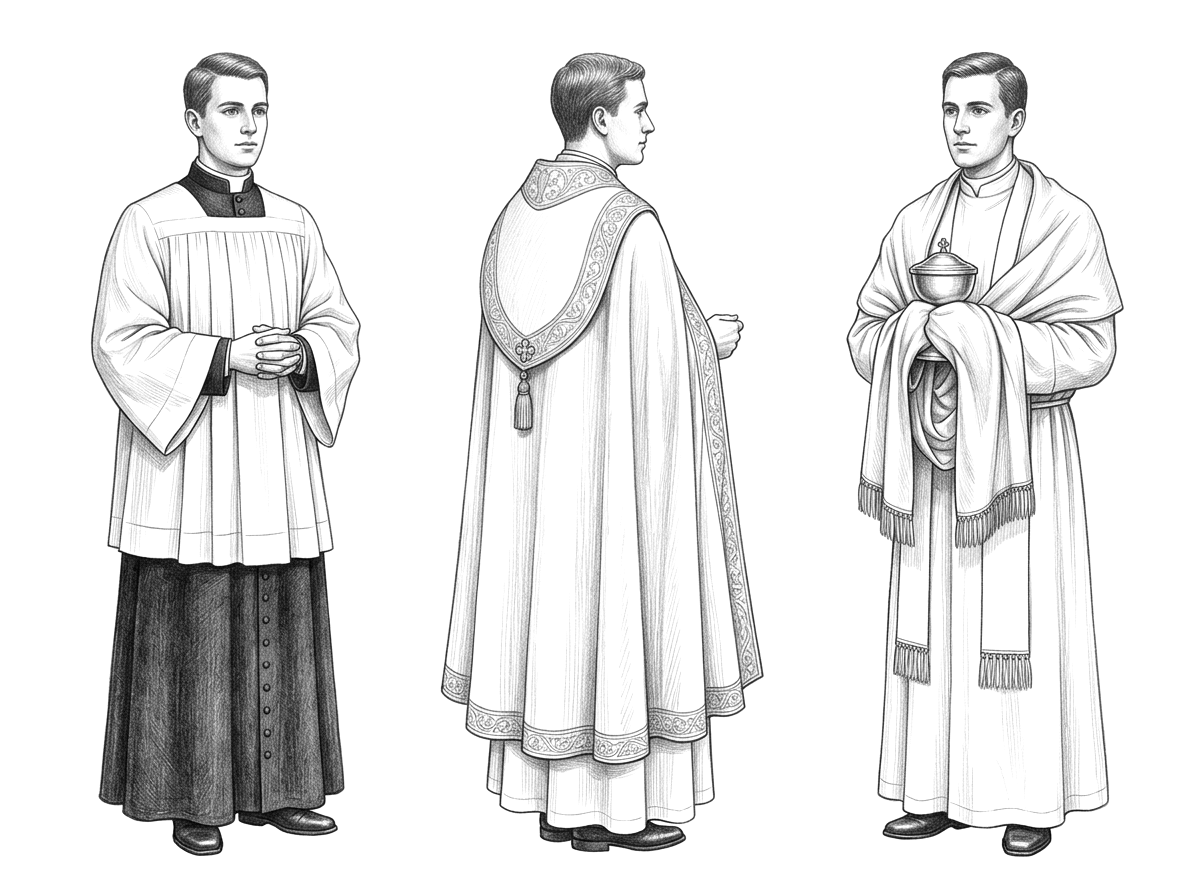
\includegraphics[width=0.92\linewidth,height=3.55in,keepaspectratio]{liturgy/roman-rite/postconciliar/2008-latin-2011-us-english/reference/roman-sanctuary-dictionary/shared/artwork/graphite/pc-art-09-black-cassock-surplice-cope.png}
\end{center}
\PCDPositionKey{Left: choir dress (deep black buttoned clerical Cassock beneath crisp white pleated Surplice); center: three-quarter rear view of semicircular Cope with ornamental hood shield and tassel over an Alb; right: Priest in Alb and straight Stole wearing a fringed Humeral Veil whose cloth completely envelops both hands supporting a closed lidded ciborium.}
\else
\textbf{Visual Plate Summary (Plate IX --- Choir Dress and Solemn Ceremonial Vesture, Standing figures to common scale):} Three-figure monochrome graphite garment study demonstrating high-contrast shading: left, a standing figure in clerical choir dress wearing a deep charcoal-black ankle-length buttoned cassock under a bright white pleated wide-sleeved surplice; center, three-quarter rear view of a flowing semicircular cope with embroidered hood shield and tassel worn over a white alb; right, three-quarter front view of a priest in alb and straight vertical stole draped in an oblong fringed humeral veil whose ends wrap completely over both hands as he holds a closed lidded ciborium.

\textbf{Reading order and object placement:} Left: choir dress (deep black buttoned clerical Cassock beneath crisp white pleated Surplice); center: three-quarter rear view of semicircular Cope with ornamental hood shield and tassel over an Alb; right: Priest in Alb and straight Stole wearing a fringed Humeral Veil whose cloth completely envelops both hands supporting a closed lidded ciborium.
\fi

\label{pc-obj-cassock-surplice}
\PCDEntryHead{Cassock and Surplice}{Vestis talaris et superpelliceum}{permitted}{N37}
\PCDField{Also called}{Choir Dress; Server's Cassock and Surplice; \textit{Talaris}; \textit{Superpelliceum}; \textit{Cotta}}
In many parishes, altar servers wear a black buttoned cassock under a crisp white pleated surplice instead of an alb---both are lawful and dignified under United States norms (US GIRM 339). Always wear the surplice over a cassock, never over street trousers or a shirt by itself (CE 1984 no. 65). Check that your cassock clears your shoes so you will not trip on sanctuary steps, wear dark modest shoes beneath it, button the cassock neatly, and hang both garments cleanly in the sacristy after Mass.

\PCDField{Where to look on the plate}{Left figure, deep charcoal-black ankle-length buttoned cassock under bright pleated white surplice (Plate IX)}
\PCDField{Handling boundary}{\textbf{Server handles directly.} Altar servers wear cassock and surplice where parish custom appoints them (US GIRM 339), always wearing the surplice over a properly fitted cassock (never over street clothes alone) and never adding clerical collars, stoles, or prelatial insignia. (Ordinary ministers: Bishop, Priest, Deacon, Instituted acolyte, Altar server.)}
\PCDSafety{Ensure the cassock hem clears the floor cleanly above the shoes so it does not catch on sanctuary steps while carrying candles, the processional cross, or a smoking thurible; never wear a surplice without a cassock underneath (CE 1984 no. 65).}
\PCDField{Do not confuse with}{Alb}
\PCDEntryRule

\label{pc-obj-cope}
\PCDEntryHead{Cope}{Pluviale}{provided}{N38}
\PCDField{Also called}{Processional Mantle; \textit{Cappa}}
You will recognize the cope immediately by its long flowing cloak shape, open down the front, with a flat shield-like hood hanging down the back. Priests and deacons wear it outside Mass---for Solemn Benediction, Eucharistic processions, and Solemn Vespers---never for offering the Mass itself. During Benediction or processions, you may be asked to hold back the front edges of the cope so the priest can freely use the thurible or lift the monstrance; keep the fabric carefully clear of open flames and glowing charcoal.

\PCDField{Where to look on the plate}{Center figure, three-quarter rear view showing full semicircular cloak, embroidered hood shield, and tassel over an alb (Plate IX)}
\PCDField{Handling boundary}{\textbf{Clergy-reserved; server does not touch.} Strictly reserved to bishops, priests, and deacons presiding at proper non-Mass rites; servers never wear a cope, though servers may assist in vesting it in the sacristy and---when directed during Benediction or processions---hold back its front edges as the celebrant incenses or blesses. (Ordinary ministers: Bishop, Priest, Deacon.)}
\PCDSafety{When holding the edges of a priest's or bishop's cope during incensation or procession, keep the heavy front fabric well clear of lighted candles and hot thurible chains, and unfasten the chest clasp gently without tugging delicate embroidery.}
\PCDField{Do not confuse with}{Chasuble, Humeral Veil}
\PCDEntryRule

\label{pc-obj-humeral-veil}
\PCDEntryHead{Humeral Veil}{Velum humerale}{provided}{N39}
\PCDField{Also called}{Benediction Veil; \textit{Velum}}
Look closely at the priest on the right of Plate IX: the fringed white humeral veil wraps completely over his hands so he holds the sacred vessel through the cloth, showing that Christ Himself gives the blessing. You will never wear this veil to hold the Blessed Sacrament, but you have an important assisting role at Benediction and on Holy Thursday: step behind the kneeling priest or deacon at the cue, drape the veil evenly over his shoulders with its center cross straight down his back, fasten the front clasp neatly, and stand clear of its fringed ends as he rises.

\PCDField{Where to look on the plate}{Right figure, oblong fringed white cloth draped over shoulders with ends wrapping completely over both hands around a lidded ciborium (Plate IX)}
\PCDField{Handling boundary}{\textbf{Server carries and presents to priest or deacon.} Servers never wear the Eucharistic humeral veil to carry or bless with the Blessed Sacrament. During Benediction or Holy Thursday transfer, a server places the humeral veil evenly across the priest's or deacon's shoulders, fastens the front clasp securely, and removes and folds it cleanly afterward. (Ordinary ministers: Bishop, Priest, Deacon.)}
\PCDSafety{Fasten the front clasp cleanly and evenly without pulling the priest's stole or collar, and ensure the long fringed ends do not brush against lighted candles on the altar steps while the celebrant ascends to lift the monstrance or ciborium.}
\PCDField{Do not confuse with}{Cope, Stole}
\PCDEntryRule

\clearpage
\PCDPlateHeader{Plate X --- Communion Under Both Kinds and Sacramental Vessels}{Not to common scale}
\ifdefined\TriptychPrintEdition
\begin{center}
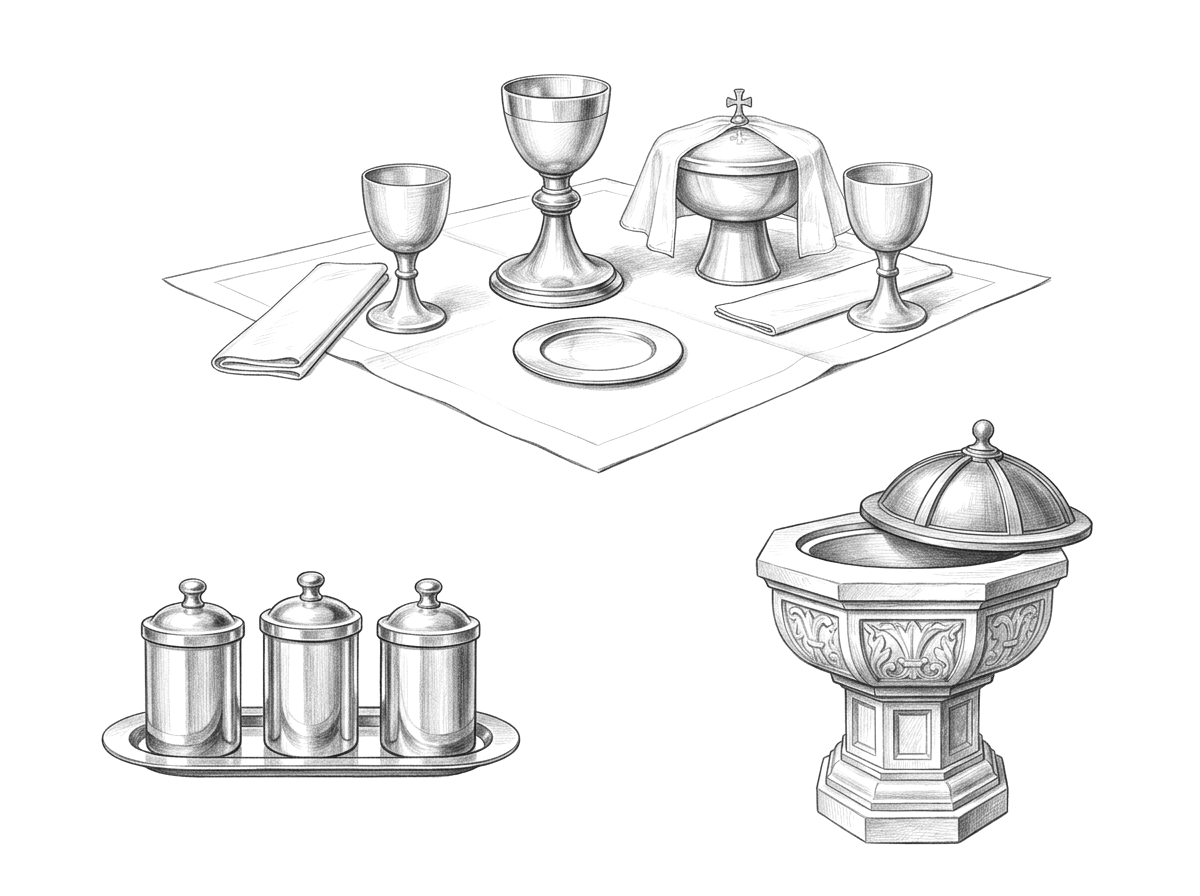
\includegraphics[width=0.92\linewidth,height=3.55in,keepaspectratio]{liturgy/roman-rite/postconciliar/2008-latin-2011-us-english/reference/roman-sanctuary-dictionary/shared/artwork/graphite/pc-art-10-communion-triduum-vessels.png}
\end{center}
\PCDPositionKey{Top: Communion under both kinds arrangement on an unfolded Corporal (principal Chalice, Paten, veiled covered Ciborium, and two footed Communion Cups each with a folded Purificator); bottom left: three cylindrical lidded metal Holy Oils Stocks on a tray (Sacred Chrism, Oil of Catechumens, Oil of the Sick); bottom right: carved octagonal stone Baptismal Font with removable domed cover ajar.}
\else
\textbf{Visual Plate Summary (Plate X --- Communion Under Both Kinds and Sacramental Vessels, Not to common scale):} Three-group monochrome graphite sacramental plate: top, an unfolded square corporal holding a central principal chalice, shallow paten, closed ciborium draped in a white veil, and two footed Communion cups each beside a folded purificator; bottom left, three matching cylindrical lidded metal holy-oil vessels resting on an oval metal tray without baked inscriptions; bottom right, an octagonal carved stone baptismal font on a pedestal with its domed cover resting slightly open to reveal the water basin rim.

\textbf{Reading order and object placement:} Top: Communion under both kinds arrangement on an unfolded Corporal (principal Chalice, Paten, veiled covered Ciborium, and two footed Communion Cups each with a folded Purificator); bottom left: three cylindrical lidded metal Holy Oils Stocks on a tray (Sacred Chrism, Oil of Catechumens, Oil of the Sick); bottom right: carved octagonal stone Baptismal Font with removable domed cover ajar.
\fi

\label{pc-obj-holy-oils-stocks}
\PCDEntryHead{Holy Oils and Oil Stocks}{Olea sancta et vasa oleorum}{required}{N40}
\PCDField{Also called}{Sacred Chrism (SC), Oil of Catechumens (OC), and Oil of the Sick (OI); oil stocks; chrismatory; oil urns; ambry (oil cabinet); \textit{Sanctum Chrisma}; \textit{Oleum catechumenorum}; \textit{Oleum infirmorum}; \textit{ampullae oleorum}; \textit{thecae}; \textit{armarium oleorum}}
You will see the three matching cylindrical oil stocks on Plate X beside the baptismal font, and in church you may see larger urns reserved behind a locked ambry door. If assigned to carry one of the closed urns during the Chrism Mass or the Holy Thursday reception of the holy oils, hold it level and steady with both hands and never loosen the lid. During Baptisms or Confirmations, you may hold a small tray with cotton, a slice of lemon, and a finger towel for the priest or bishop to cleanse his hands after anointing, while leaving the stocks themselves strictly to the ordained minister.

\PCDField{Where to look on the plate}{Bottom left, three matching cylindrical lidded metal oil stocks on an oval tray (Plate X)}
\PCDField{Handling boundary}{\textbf{Server moves only at celebrant's or sacristan's direction.} Carry closed oil urns in procession only when designated (such as at the Chrism Mass or Holy Thursday reception of the oils) and hold a service tray with cotton and towel for the minister during Baptism or Confirmation; never open a stock, anoint anyone, transpose caps, or handle the ambry key. (Ordinary ministers: Bishop, Priest, Deacon.)}
\PCDSafety{Never open an oil stock, attempt to anoint anyone, or interchange caps between SC, OC, and OI vessels. Hold closed oil urns upright with both hands during processions to prevent oil spills on sanctuary steps, and never discard previous year's oils in ordinary sinks, trash, or plumbing; old oils are burned reverently (commonly absorbed in cotton or consumed in the Easter fire) or poured into the sacrarium or clean earth according to diocesan direction.}
\PCDField{Do not confuse with}{Pyx, Cruets}
\PCDEntryRule
